\documentclass[aspectratio=169,14pt]{beamer}

% NeurIPS color scheme
\usepackage{xcolor}
\definecolor{primary}{HTML}{8B5CF6}
\definecolor{accent}{HTML}{2563EB}
\definecolor{darktext}{HTML}{1E1E1E}
\definecolor{lightgray}{HTML}{F3F4F6}
\definecolor{wingreen}{HTML}{059669}
\definecolor{losered}{HTML}{DC2626}

% Theme
\usetheme{default}
\usecolortheme{default}
\setbeamercolor{frametitle}{fg=primary}
\setbeamercolor{title}{fg=primary}
\setbeamercolor{structure}{fg=accent}
\setbeamercolor{itemize item}{fg=primary}
\setbeamercolor{itemize subitem}{fg=accent}
\setbeamercolor{block title}{bg=primary!15,fg=primary}
\setbeamercolor{block body}{bg=primary!5}
\setbeamertemplate{navigation symbols}{}
\setbeamertemplate{footline}{
  \hfill\usebeamercolor[fg]{frametitle}\scriptsize\insertframenumber/\inserttotalframenumber\hspace{3mm}\vspace{2mm}
}
\setbeamerfont{frametitle}{size=\Large,series=\bfseries}

% Packages
\usepackage{graphicx,amsmath,booktabs,multirow,array,tikz}
\usepackage{fontenc}

% Metadata
\title{\textbf{Multi-View Internal State Fusion\\for LLM Probing}}
\subtitle{NeurIPS 2026 Progress Report}
\author{Junyi Chen}
\date{April 2026}

\begin{document}

% ============================================================
% Slide 1: Title
% ============================================================
\begin{frame}
\titlepage
\end{frame}

% ============================================================
% Slide 2: Motivation
% ============================================================
\begin{frame}{Motivation: A Fragmented Landscape}

\begin{columns}[T]
\begin{column}{0.55\textwidth}
\textbf{Problem}: 12+ probing methods exist, each:
\begin{itemize}
    \item Extracts \textbf{different} internal signals
    \item Evaluates on \textbf{different} datasets
    \item Uses \textbf{different} layers/representations
\end{itemize}

\vspace{1em}
\textcolor{primary}{\textbf{Gap}}: Nobody has systematically\\
fused multiple probing methods.

\vspace{0.5em}
{\small Confirmed by RepE Survey (2025), PING (2025)}
\end{column}

\begin{column}{0.42\textwidth}
\centering
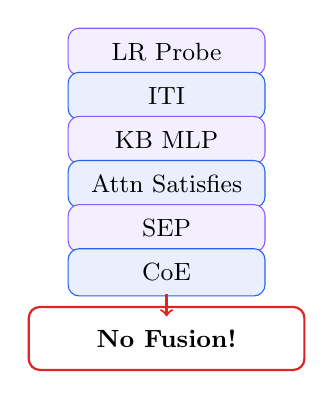
\begin{tikzpicture}[scale=0.7]
\node[draw=primary, rounded corners, fill=primary!10, minimum width=2.5cm, minimum height=0.6cm] at (0,3) {\small LR Probe};
\node[draw=accent, rounded corners, fill=accent!10, minimum width=2.5cm, minimum height=0.6cm] at (0,2.2) {\small ITI};
\node[draw=primary, rounded corners, fill=primary!10, minimum width=2.5cm, minimum height=0.6cm] at (0,1.4) {\small KB MLP};
\node[draw=accent, rounded corners, fill=accent!10, minimum width=2.5cm, minimum height=0.6cm] at (0,0.6) {\small Attn Satisfies};
\node[draw=primary, rounded corners, fill=primary!10, minimum width=2.5cm, minimum height=0.6cm] at (0,-0.2) {\small SEP};
\node[draw=accent, rounded corners, fill=accent!10, minimum width=2.5cm, minimum height=0.6cm] at (0,-1.0) {\small CoE};
\node[draw=losered, thick, rounded corners, minimum width=3.5cm, minimum height=0.8cm] at (0,-2.2) {\small \textbf{No Fusion!}};
\draw[->, thick, losered] (0,-1.4) -- (0,-1.8);
\end{tikzpicture}
\end{column}
\end{columns}

\end{frame}

% ============================================================
% Slide 3: Project Pipeline
% ============================================================
\begin{frame}{Project Pipeline}

\centering
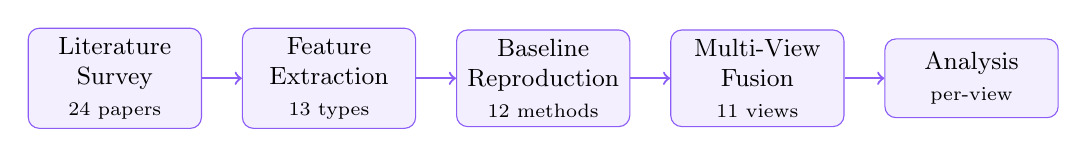
\begin{tikzpicture}[
    box/.style={draw=primary, rounded corners, fill=primary!10, minimum width=2.2cm, minimum height=1cm, align=center, font=\small},
    arr/.style={->, thick, primary},
    scale=0.85
]
\node[box] (s1) at (0,0) {Literature\\Survey\\{\scriptsize 24 papers}};
\node[box] (s2) at (3.2,0) {Feature\\Extraction\\{\scriptsize 13 types}};
\node[box] (s3) at (6.4,0) {Baseline\\Reproduction\\{\scriptsize 12 methods}};
\node[box] (s4) at (9.6,0) {Multi-View\\Fusion\\{\scriptsize 11 views}};
\node[box] (s5) at (12.8,0) {Analysis\\{\scriptsize per-view}};

\draw[arr] (s1) -- (s2);
\draw[arr] (s2) -- (s3);
\draw[arr] (s3) -- (s4);
\draw[arr] (s4) -- (s5);
\end{tikzpicture}

\vspace{1.5em}

\begin{columns}[T]
\begin{column}{0.3\textwidth}
\centering
\textbf{Data Scale}\\
27,948 samples\\
392 GB features\\
9 datasets
\end{column}
\begin{column}{0.3\textwidth}
\centering
\textbf{Model}\\
Qwen2.5-7B-Instruct\\
2-pass extraction\\
2$\times$A100
\end{column}
\begin{column}{0.3\textwidth}
\centering
\textbf{Tasks}\\
Factuality, Routing\\
Hallucination\\
Difficulty prediction
\end{column}
\end{columns}

\end{frame}

% ============================================================
% Slide 4: Baseline Reproduction
% ============================================================
\begin{frame}{12 Methods Faithfully Reproduced}

\small
\begin{columns}[T]
\begin{column}{0.48\textwidth}
\textbf{Hidden State Probing} (dominate)
\begin{itemize}
    \item LR Probe {\scriptsize (COLM'24)}
    \item PCA+LR {\scriptsize (arXiv'25)}
    \item ITI {\scriptsize (NeurIPS'23)}
    \item KB MLP {\scriptsize (ACL'25)}
\end{itemize}

\textbf{Attention-based}
\begin{itemize}
    \item Attn Satisfies {\scriptsize (ICLR'24)}
    \item LLM-Check {\scriptsize (NeurIPS'24)}
\end{itemize}
\end{column}

\begin{column}{0.48\textwidth}
\textbf{Generation-based}
\begin{itemize}
    \item SEP {\scriptsize (arXiv'24)}
    \item STEP {\scriptsize (ICLR'25)}
    \item MM Probe {\scriptsize (COLM'24)}
\end{itemize}

\textbf{Unsupervised} ($\approx$ random)
\begin{itemize}
    \item CoE {\scriptsize (ICLR'25)}
    \item SeaKR {\scriptsize (ACL'25)}
    \item LID {\scriptsize (arXiv'24)}
\end{itemize}
\end{column}
\end{columns}

\vspace{0.8em}
\centering
\textcolor{primary}{\textbf{Key finding}}: Hidden state probes dominate. Unsupervised methods near random.

\end{frame}

% ============================================================
% Slide 5: Oracle — Probes are Complementary
% ============================================================
\begin{frame}{Key Finding: Probes Make \textit{Different} Errors}

\centering
\textbf{Per-example oracle} (pick best probe per sample):

\vspace{0.5em}
\begin{tabular}{l c c c}
\toprule
\textbf{Dataset} & \textbf{Best Single} & \textbf{Oracle} & \textbf{Headroom} \\
\midrule
common\_claim & 0.771 & \textbf{0.979} & \textcolor{wingreen}{\textbf{+20.8\%}} \\
when2call & 0.864 & \textbf{0.990} & \textcolor{wingreen}{\textbf{+12.6\%}} \\
ragtruth & 0.880 & \textbf{1.000} & \textcolor{wingreen}{\textbf{+11.9\%}} \\
fava & 0.985 & \textbf{1.000} & \textcolor{wingreen}{\textbf{+1.5\%}} \\
\bottomrule
\end{tabular}

\vspace{1.5em}
\textcolor{primary}{\textbf{12--21\% headroom}} $\Rightarrow$ probes are genuinely complementary\\
\vspace{0.3em}
{\small Question: Can we capture this complementarity with simple fusion?}

\end{frame}

% ============================================================
% Slide 6: Method — MVISF-v2
% ============================================================
\begin{frame}{Method: Multi-View Internal State Fusion}

\centering
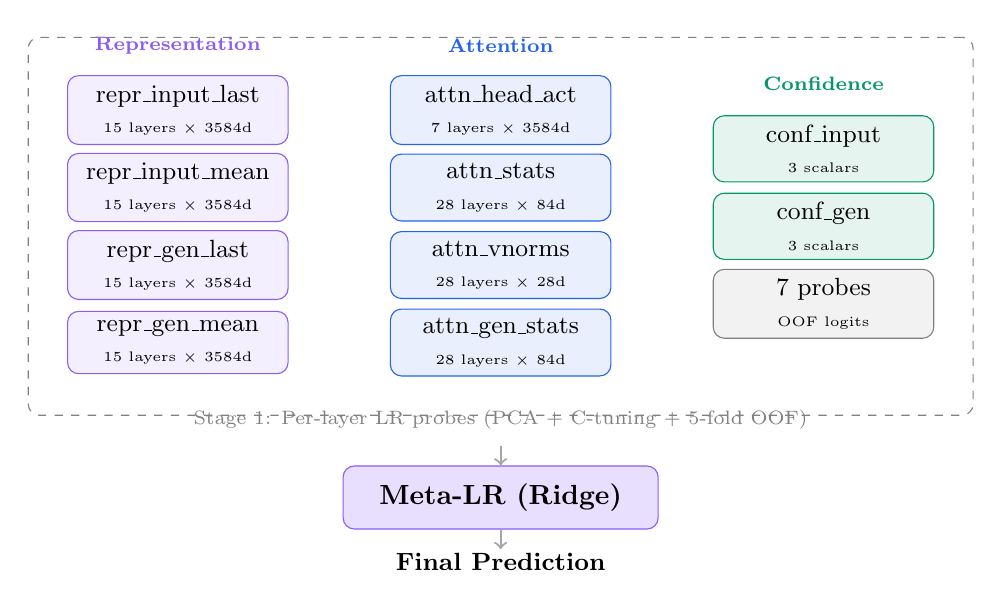
\begin{tikzpicture}[
    vp/.style={draw=primary, rounded corners, fill=primary!10, minimum width=2.8cm, minimum height=0.7cm, align=center, font=\small},
    va/.style={draw=accent, rounded corners, fill=accent!10, minimum width=2.8cm, minimum height=0.7cm, align=center, font=\small},
    vc/.style={draw=wingreen, rounded corners, fill=wingreen!10, minimum width=2.8cm, minimum height=0.7cm, align=center, font=\small},
    vg/.style={draw=gray, rounded corners, fill=gray!10, minimum width=2.8cm, minimum height=0.7cm, align=center, font=\small},
    meta/.style={draw=primary, rounded corners, fill=primary!20, minimum width=4cm, minimum height=0.8cm, align=center, font=\normalsize\bfseries},
    arr/.style={->, thick, gray!70},
    scale=0.82
]
% Views
\node[vp] (v1) at (-5, 2.0) {repr\_input\_last\\{\tiny 15 layers $\times$ 3584d}};
\node[vp] (v2) at (-5, 0.8) {repr\_input\_mean\\{\tiny 15 layers $\times$ 3584d}};
\node[vp] (v3) at (-5, -0.4) {repr\_gen\_last\\{\tiny 15 layers $\times$ 3584d}};
\node[vp] (v4) at (-5, -1.6) {repr\_gen\_mean\\{\tiny 15 layers $\times$ 3584d}};

\node[va] (v5) at (0, 2.0) {attn\_head\_act\\{\tiny 7 layers $\times$ 3584d}};
\node[va] (v6) at (0, 0.8) {attn\_stats\\{\tiny 28 layers $\times$ 84d}};
\node[va] (v7) at (0, -0.4) {attn\_vnorms\\{\tiny 28 layers $\times$ 28d}};
\node[va] (v8) at (0, -1.6) {attn\_gen\_stats\\{\tiny 28 layers $\times$ 84d}};

\node[vc] (v9) at (5, 1.4) {conf\_input\\{\tiny 3 scalars}};
\node[vc] (v10) at (5, 0.2) {conf\_gen\\{\tiny 3 scalars}};
\node[vg] (v11) at (5, -1.0) {7 probes\\{\tiny OOF logits}};

% Stage labels
\node[font=\scriptsize\bfseries, primary] at (-5, 3.0) {Representation};
\node[font=\scriptsize\bfseries, accent] at (0, 3.0) {Attention};
\node[font=\scriptsize\bfseries, wingreen] at (5, 2.4) {Confidence};

% Per-layer LR
\node[draw=gray, dashed, rounded corners, minimum width=12cm, minimum height=4.8cm] at (0, 0.2) {};
\node[font=\scriptsize, gray] at (0, -2.8) {Stage 1: Per-layer LR probes (PCA + C-tuning + 5-fold OOF)};

% Meta
\node[meta] (final) at (0, -4.0) {Meta-LR (Ridge)};
\draw[arr] (0, -3.2) -- (final);

% Output
\node[font=\small\bfseries] at (0, -5.0) {Final Prediction};
\draw[arr] (final) -- (0, -4.8);

\end{tikzpicture}

\end{frame}

% ============================================================
% Slide 7: View Taxonomy
% ============================================================
\begin{frame}{View Taxonomy: 4 Computational Perspectives}

\begin{columns}[T]
\begin{column}{0.48\textwidth}

\textbf{\textcolor{primary}{Representation}} — \textit{What it represents}
\begin{itemize}
    \item Last-token hidden states (input/gen)
    \item \textbf{Mean-pooled} hidden states (input/gen)
    \item {\small $\rightarrow$ 4 views, 60 layers total}
\end{itemize}

\vspace{0.5em}
\textbf{\textcolor{accent}{Attention}} — \textit{Where it looks}
\begin{itemize}
    \item Per-head activations
    \item Attention stats (skew, entropy)
    \item Value norms
    \item {\small $\rightarrow$ 4 views, 91 layers total}
\end{itemize}

\end{column}
\begin{column}{0.48\textwidth}

\textbf{\textcolor{wingreen}{Confidence}} — \textit{How certain it is}
\begin{itemize}
    \item Input logit stats (entropy, max\_prob)
    \item Gen logit stats
    \item {\small $\rightarrow$ 2 views, 6 scalars total}
\end{itemize}

\vspace{0.5em}
\textbf{Probe} — \textit{Published methods}
\begin{itemize}
    \item 7 reproduced probing methods
    \item OOF logits as features
    \item {\small $\rightarrow$ 1 view, 7 probe outputs}
\end{itemize}

\vspace{0.5em}
{\small \textcolor{primary}{\textbf{5 of 11 views are NEW}} (previously unused features)}

\end{column}
\end{columns}

\end{frame}

% ============================================================
% Slide 8: Main Results
% ============================================================
\begin{frame}{Results: 7/7 Non-Saturated Datasets Improved}

\centering
\small
\begin{tabular}{l c c r l}
\toprule
\textbf{Dataset} & \textbf{Best Single} & \textbf{MVISF-v2} & \textbf{$\Delta$} & \textbf{95\% CI} \\
\midrule
GoT Cities & 1.000 & 0.999 & \textcolor{gray}{-0.07\%} & {\scriptsize [.998, 1.00] \textcolor{gray}{saturated}} \\
MetaTool & 0.998 & 0.996 & \textcolor{gray}{-0.25\%} & {\scriptsize [.989, 1.00] \textcolor{gray}{saturated}} \\
\midrule
RetrievalQA & 0.939 & \textbf{0.946} & \textcolor{wingreen}{+0.66\%} & {\scriptsize [.929, .963]} \\
common\_claim & 0.758 & \textbf{0.776} & \textcolor{wingreen}{+1.88\%} & {\scriptsize [.753, .800]} \\
E2H AMC 3c & 0.893 & \textbf{0.914} & \textcolor{wingreen}{+2.06\%} & {\scriptsize [.907, .921]} \\
E2H AMC 5c & 0.875 & \textbf{0.898} & \textcolor{wingreen}{+2.28\%} & {\scriptsize [.891, .904]} \\
\textbf{When2Call} & 0.874 & \textbf{0.938} & \textcolor{wingreen}{\textbf{+6.41\%}} & {\scriptsize [.925, .952]} \\
FAVA & 0.986 & \textbf{0.991} & \textcolor{wingreen}{+0.51\%} & {\scriptsize [.986, .995]} \\
RAGTruth & 0.881 & \textbf{0.885} & \textcolor{wingreen}{+0.42\%} & {\scriptsize [.864, .906]} \\
\bottomrule
\end{tabular}

\vspace{0.8em}
\textbf{Wilcoxon signed-rank: $p = 0.0098$} {\small (significant at 1\%)}

\end{frame}

% ============================================================
% Slide 9: When2Call Highlight
% ============================================================
\begin{frame}{Highlight: When2Call +6.41\%}

\begin{columns}[T]
\begin{column}{0.55\textwidth}
\textbf{Task}: 3-class tool routing\\
{\small (no tool / calculator / search engine)}

\vspace{1em}
\textbf{Why so large?}
\begin{itemize}
    \item \texttt{repr\_input\_mean} alone: \textbf{0.933}
    \item \texttt{repr\_input\_last} alone: 0.904
    \item Gap: \textcolor{wingreen}{\textbf{+2.9\%}}
\end{itemize}

\vspace{0.5em}
Mean-pooled representations capture\\
\textbf{global prompt context} that\\
last-token misses for routing decisions.

\end{column}
\begin{column}{0.42\textwidth}

\centering
\textbf{LOO Contributions}

\vspace{0.5em}
\begin{tabular}{l r}
\toprule
\textbf{View} & \textbf{$\Delta$} \\
\midrule
repr\_input\_mean & \textcolor{wingreen}{\textbf{+2.26\%}} \\
repr\_input\_last & +0.46\% \\
repr\_gen\_mean & +0.17\% \\
attn\_head\_act & +0.12\% \\
probe\_methods & +0.07\% \\
\midrule
\textit{Others} & \textit{$\leq$0} \\
\bottomrule
\end{tabular}

\end{column}
\end{columns}

\end{frame}

% ============================================================
% Slide 10: Per-View Analysis
% ============================================================
\begin{frame}{Per-View Contribution Analysis}

\begin{columns}[T]
\begin{column}{0.48\textwidth}
\textbf{Avg standalone AUROC}\\{\small (across 9 datasets)}

\vspace{0.3em}
\small
\begin{tabular}{l r}
\toprule
\textbf{View} & \textbf{AUROC} \\
\midrule
repr\_input\_last & 0.921 \\
attn\_head\_act & 0.919 \\
\textcolor{primary}{\textbf{repr\_input\_mean}} & \textcolor{primary}{\textbf{0.907}} \\
attn\_input\_stats & 0.892 \\
probe\_methods & 0.891 \\
attn\_input\_vnorms & 0.872 \\
\textcolor{primary}{repr\_gen\_mean} & \textcolor{primary}{0.868} \\
attn\_gen\_stats & 0.794 \\
repr\_gen\_last & 0.732 \\
conf\_input & 0.683 \\
conf\_gen & 0.558 \\
\bottomrule
\end{tabular}
\end{column}

\begin{column}{0.48\textwidth}
\textbf{Avg LOO contribution}\\{\small (how much removing it hurts)}

\vspace{0.3em}
\small
\begin{tabular}{l r}
\toprule
\textbf{View} & \textbf{Contrib.} \\
\midrule
\textcolor{primary}{\textbf{repr\_input\_mean}} & \textcolor{wingreen}{\textbf{+0.0030}} \\
probe\_methods & +0.0020 \\
repr\_input\_last & +0.0007 \\
repr\_gen\_mean & +0.0005 \\
attn\_head\_act & +0.0004 \\
\midrule
repr\_gen\_last & +0.0000 \\
attn\_input\_vnorms & -0.0000 \\
attn\_input\_stats & -0.0002 \\
conf\_gen & -0.0002 \\
conf\_input & -0.0005 \\
attn\_gen\_stats & -0.0005 \\
\bottomrule
\end{tabular}
\end{column}
\end{columns}

\vspace{0.5em}
\centering
{\small \textcolor{primary}{\textbf{repr\_input\_mean}} = \#1 complementary signal (previously unused!)}

\end{frame}

% ============================================================
% Slide 11: Scientific Insights
% ============================================================
\begin{frame}{Scientific Insights}

\textbf{1. Mean-pooled prompt representations are underexplored}
\begin{itemize}
    \item All 12 baselines use \textbf{last-token} or \textbf{per-token} probing
    \item Mean-pool captures \textbf{global context} $\rightarrow$ strongest complementary signal
    \item Task-dependent: routing (+2.3\%) $\gg$ factuality (+0.1\%)
\end{itemize}

\vspace{0.8em}
\textbf{2. View contribution is task-dependent}
\begin{itemize}
    \item Tool routing: mean-pool dominates
    \item Hallucination: probe methods + attention
    \item Difficulty prediction: input hidden + head activations
\end{itemize}

\vspace{0.8em}
\textbf{3. Linear fusion is optimal in low-data probing}
\begin{itemize}
    \item Neural fusion (493K params): \textcolor{losered}{-2\% to -9\%}
    \item Linear stacking (few K params): \textcolor{wingreen}{+0.4\% to +6.4\%}
    \item Sweet spot for 800--3500 samples
\end{itemize}

\end{frame}

% ============================================================
% Slide 12: Review Progression
% ============================================================
\begin{frame}{GPT-5.4 Review Loop: 4/10 $\rightarrow$ 8/10}

\centering
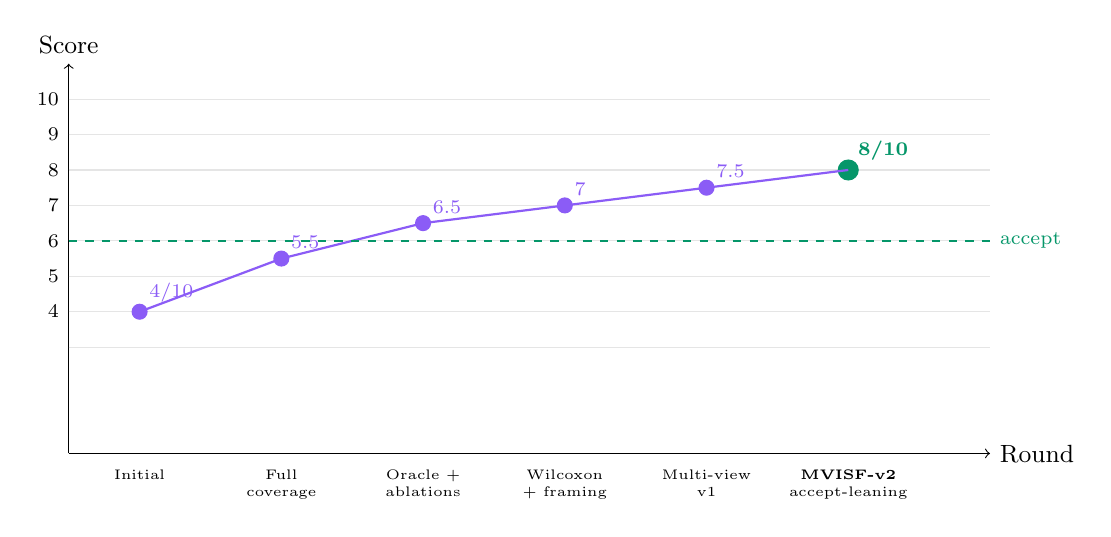
\begin{tikzpicture}[scale=0.9]
\draw[->] (0,0) -- (13,0) node[right] {\small Round};
\draw[->] (0,0) -- (0,5.5) node[above] {\small Score};

% Grid
\draw[gray!20] (0,1.5) -- (13,1.5);
\draw[gray!20] (0,2) -- (13,2);
\draw[gray!20] (0,2.5) -- (13,2.5);
\draw[gray!20] (0,3) -- (13,3);
\draw[gray!20] (0,3.5) -- (13,3.5);
\draw[gray!20] (0,4) -- (13,4);
\draw[gray!20] (0,4.5) -- (13,4.5);
\draw[gray!20] (0,5) -- (13,5);

% Y labels
\node[left, font=\scriptsize] at (0,2) {4};
\node[left, font=\scriptsize] at (0,2.5) {5};
\node[left, font=\scriptsize] at (0,3) {6};
\node[left, font=\scriptsize] at (0,3.5) {7};
\node[left, font=\scriptsize] at (0,4) {8};
\node[left, font=\scriptsize] at (0,4.5) {9};
\node[left, font=\scriptsize] at (0,5) {10};

% Data points
\filldraw[primary] (1,2) circle (3pt) node[above right, font=\scriptsize] {4/10};
\filldraw[primary] (3,2.75) circle (3pt) node[above right, font=\scriptsize] {5.5};
\filldraw[primary] (5,3.25) circle (3pt) node[above right, font=\scriptsize] {6.5};
\filldraw[primary] (7,3.5) circle (3pt) node[above right, font=\scriptsize] {7};
\filldraw[primary] (9,3.75) circle (3pt) node[above right, font=\scriptsize] {7.5};
\filldraw[wingreen] (11,4) circle (4pt) node[above right, font=\scriptsize\bfseries] {\textcolor{wingreen}{8/10}};

\draw[primary, thick] (1,2) -- (3,2.75) -- (5,3.25) -- (7,3.5) -- (9,3.75) -- (11,4);

% Annotations
\node[below, font=\tiny, align=center] at (1,-0.1) {Initial};
\node[below, font=\tiny, align=center] at (3,-0.1) {Full\\coverage};
\node[below, font=\tiny, align=center] at (5,-0.1) {Oracle +\\ablations};
\node[below, font=\tiny, align=center] at (7,-0.1) {Wilcoxon\\+ framing};
\node[below, font=\tiny, align=center] at (9,-0.1) {Multi-view\\v1};
\node[below, font=\tiny, align=center] at (11,-0.1) {\textbf{MVISF-v2}\\accept-leaning};

% Threshold line
\draw[dashed, wingreen, thick] (0,3) -- (13,3);
\node[right, font=\scriptsize, wingreen] at (13,3) {accept};
\end{tikzpicture}

\end{frame}

% ============================================================
% Slide 13: Limitations & Next Steps
% ============================================================
\begin{frame}{Limitations \& Next Steps}

\textbf{Current limitation}
\begin{itemize}
    \item Single model: Qwen2.5-7B-Instruct only
    \item {\small GPT reviewer: ``This is the only thing between 8/10 and 9/10''}
\end{itemize}

\vspace{1em}
\textbf{Next steps}
\begin{enumerate}
    \item \textbf{Paper writing} — method + experiments + analysis ready
    \item \textbf{Second model} — Llama-3-8B or Qwen2.5-3B (needs GPU)
    \item \textbf{Regression / multi-label} — extend beyond classification
    \item \textbf{Deeper analysis} — layer-wise patterns, error case studies
\end{enumerate}

\vspace{1em}
\textbf{Target}: NeurIPS 2026 (deadline $\sim$May)

\end{frame}

% ============================================================
% Slide 14: Thank You
% ============================================================
\begin{frame}{}
\centering
\vspace{2em}
{\Huge\textcolor{primary}{\textbf{Thank You}}}

\vspace{2em}
{\Large Questions?}

\vspace{2em}
{\small
12 methods $\times$ 9 datasets $\times$ 11 views\\[0.3em]
7/7 non-saturated wins \ | \ Wilcoxon $p=0.0098$\\[0.3em]
Code: \texttt{github.com/JunyiChen-ai/NIPS2026}
}
\end{frame}

\end{document}
